%\title{LaTeX Portrait Poster Template}
%%%%%%%%%%%%%%%%%%%%%%%%%%%%%%%%%%%%%%%%%
% a0poster Portrait Poster
% LaTeX Template
% Version 1.0 (22/06/13)
%
% The a0poster class was created by:
% Gerlinde Kettl and Matthias Weiser (tex@kettl.de)
% 
% This template has been downloaded from:
% http://www.LaTeXTemplates.com
%
% License:
% CC BY-NC-SA 3.0 (http://creativecommons.org/licenses/by-nc-sa/3.0/)
%
%%%%%%%%%%%%%%%%%%%%%%%%%%%%%%%%%%%%%%%%%

%----------------------------------------------------------------------------------------
%	PACKAGES AND OTHER DOCUMENT CONFIGURATIONS
%----------------------------------------------------------------------------------------

\documentclass[a0,portrait]{a0poster}

\usepackage{multicol} % This is so we can have multiple columns of text side-by-side
\columnsep=100pt % This is the amount of white space between the columns in the poster
\columnseprule=3pt % This is the thickness of the black line between the columns in the poster

\usepackage[svgnames]{xcolor} % Specify colors by their 'svgnames', for a full list of all colors available see here: http://www.latextemplates.com/svgnames-colors

\usepackage{times} % Use the times font
%\usepackage{palatino} % Uncomment to use the Palatino font

\usepackage{graphicx} % Required for including images
\graphicspath{{figures/}} % Location of the graphics files
\usepackage{booktabs} % Top and bottom rules for table
\usepackage[font=small,labelfont=bf]{caption} % Required for specifying captions to tables and figures
\usepackage{amsfonts, amsmath, amsthm, amssymb} % For math fonts, symbols and environments
\usepackage{wrapfig} % Allows wrapping text around tables and figures

\begin{document}

%----------------------------------------------------------------------------------------
%	POSTER HEADER 
%----------------------------------------------------------------------------------------

% The header is divided into two boxes:
% The first is 75% wide and houses the title, subtitle, names, university/organization and contact information
% The second is 25% wide and houses a logo for your university/organization or a photo of you
% The widths of these boxes can be easily edited to accommodate your content as you see fit

\begin{minipage}[b]{0.75\linewidth}
\veryHuge \color{NavyBlue} \textbf{Automatically extracting synonyms in Brazilian Portuguese} \color{DarkSlateGray}\\ % Title
\Huge\textit{}\\[2cm] % Subtitle
\huge \textbf{Bruno Ferrari Guide}\\[0.5cm] % Author(s)
\huge University of Sao Paulo, Department of Linguistics\\[0.4cm] % University/organization
\Large \texttt{bruno.fguide@gmail.com}\\
\end{minipage}
%
\begin{minipage}[b]{0.25\linewidth}

\includegraphics[width=20cm]{Propor-Logos.png}\\
\end{minipage}

\vspace{1cm} % A bit of extra whitespace between the header and poster content

%----------------------------------------------------------------------------------------

\begin{multicols}{2} % This is how many columns your poster will be broken into, a portrait poster is generally split into 2 columns

%----------------------------------------------------------------------------------------
%	ABSTRACT
%----------------------------------------------------------------------------------------

\color{Navy} % Navy color for the abstract

\begin{abstract}

While new models to represent meaning as multidimensional vectors (word embedding models) such as Word2Vec \cite{mikolov2013} are consistently accurate to determine measures such as meaning similarity and relatedness between words, those models are not efficient to identify if two words are related because they have the same meaning (synonyms), the opposite meaning (antonyms) or some group relation (such as hyponyms and hypernyms). The main goal of this research is to investigate the way vector models work to represent meaning, how they are limited and if their capacities can be complemented with other approaches in order to enrich the way they represent meaning. We will work not only by methodically describing the linguistic meaning and the vector representation of it, but also by testing several different tools, such as WordNet, in a pipeline to see if substantial results in identifying synonyms can be obtained in an efficient way. This task will also require compiling a corpus of Synonym identification in Brazilian Portuguese.


\end{abstract}



%----------------------------------------------------------------------------------------
%	OBJECTIVES
%----------------------------------------------------------------------------------------

\color{DarkSlateGray} % DarkSlateGray color for the rest of the content

\section*{Main Objectives}

\begin{enumerate}
\item Have a solid understanding of how word embedding models (CBoW and SG) work and which linguistic models are beneath them.
\item Identify which linguistic limitations are inherent to the models.
\item Explore possible linguistic knowledge databases which can improve synonym extraction, such as WordNet, dictionaries, thesauri.
\item Combine different linguistic databases to improve their depth. (For instance, using Portuguese Dictionaries to improve Wordnet in a semi-supervised way).
\item Create a corpus to specifically deal with the Synonym Extraction in Portuguese.
\item Test different models to achieve a new standard for this task in Portuguese.

\end{enumerate}

%----------------------------------------------------------------------------------------
%	MATERIALS AND METHODS
%----------------------------------------------------------------------------------------

\section*{Word Embeddings and Synonym}

\begin{itemize}
\item Word embedding models represent meaning through projecting words in a Cartesian space using patterns of co-occurence.\\
\end{itemize}
\begin{center}\vspace{1cm}
	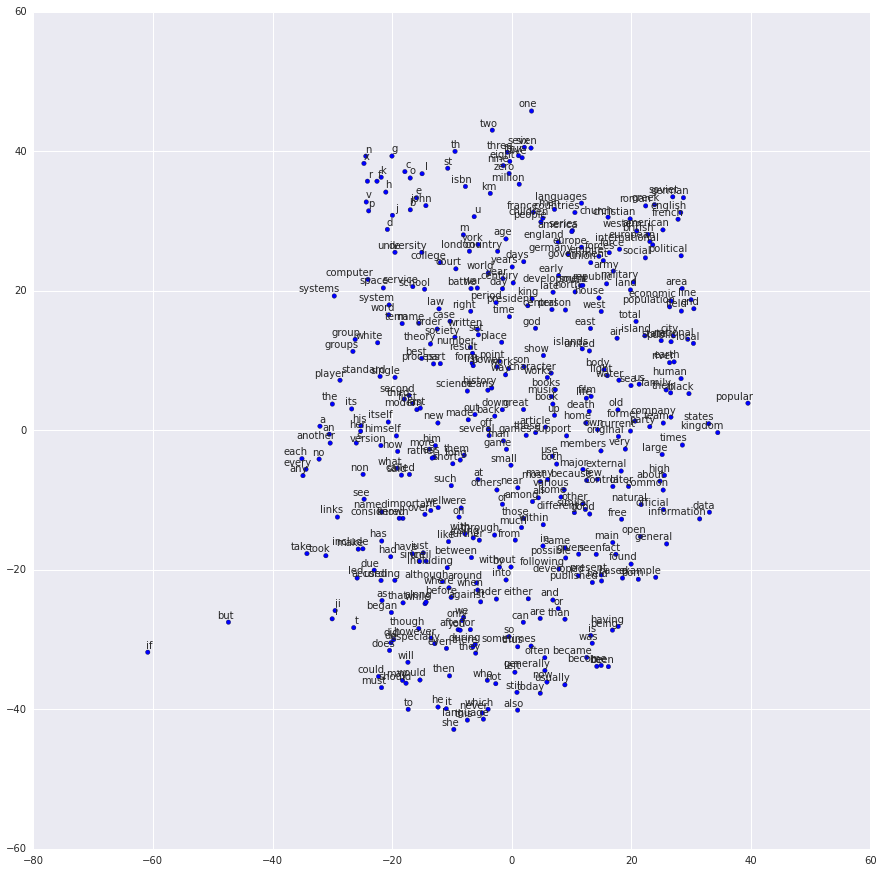
\includegraphics[width=0.8\linewidth]{w2v.png}
	\captionof{figure}{\color{Green} Word2Vec represented in a 2-dimensional space}
\end{center}\vspace{1cm}

\begin{itemize}
	\item It is possible to use linear measurements to identify relationships between those representations, those measurements tend to represent semantic relatedness in some level, such as those presented in figure 2.\\
\end{itemize}

\begin{center}\vspace{1cm}
	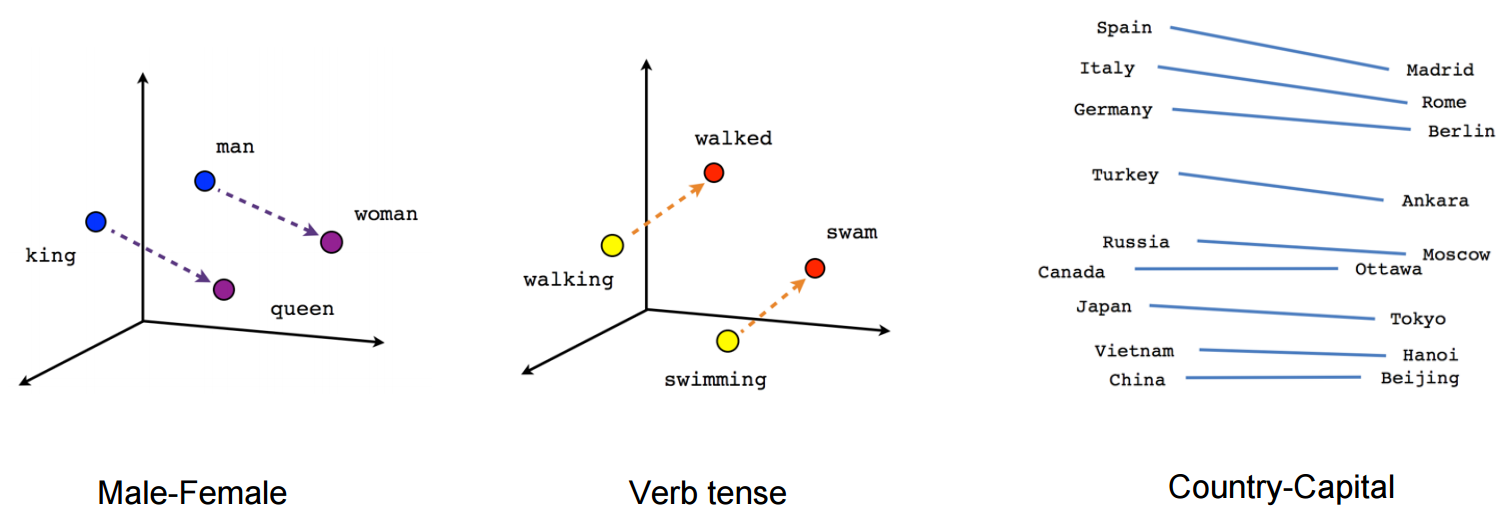
\includegraphics[width=0.8\linewidth]{linear-relationships.png}
	\captionof{figure}{\color{Green} Linear relanshionships between words in word embedding models.}
\end{center}\vspace{1cm}


\begin{itemize} 
	\item there is one caveat, several different kinds of semantic relationships are identified at the same time without any distinction, which is problematic when those different relations result in entirely different interpretations of some sentence. \\
	\item Synonym, the relationship between words which share their meaning, is especially important to not be mixed with others since it is a useful relation to several NLP tasks such as automatic translation and summarization.
	\item It is important to reiterate that this work considers that it is possible to enrich word embeddings in a way that they serve as a base to more complex models which are able to differentiate between relatedness and synonym. \\
	\item Those models are not necessarily going to be hardwired to identify a previously defined set of synonyms, we aim to find semi-supervised or non-supervised tactics to extract synonyms from the vector space.\\
\end{itemize}

%----------------------------------------------------------------------------------------
%	RESULTS 
%----------------------------------------------------------------------------------------

\section*{Ideas and Issues}
\begin{itemize}
	\item One major issue is one regarding the ambiguous structure of language itself. There are words which are not synonyms of themselves. This is the case of polysemic words such as \textit{mouse}:
%
\end{itemize}

\begin{center}\vspace{1cm}
	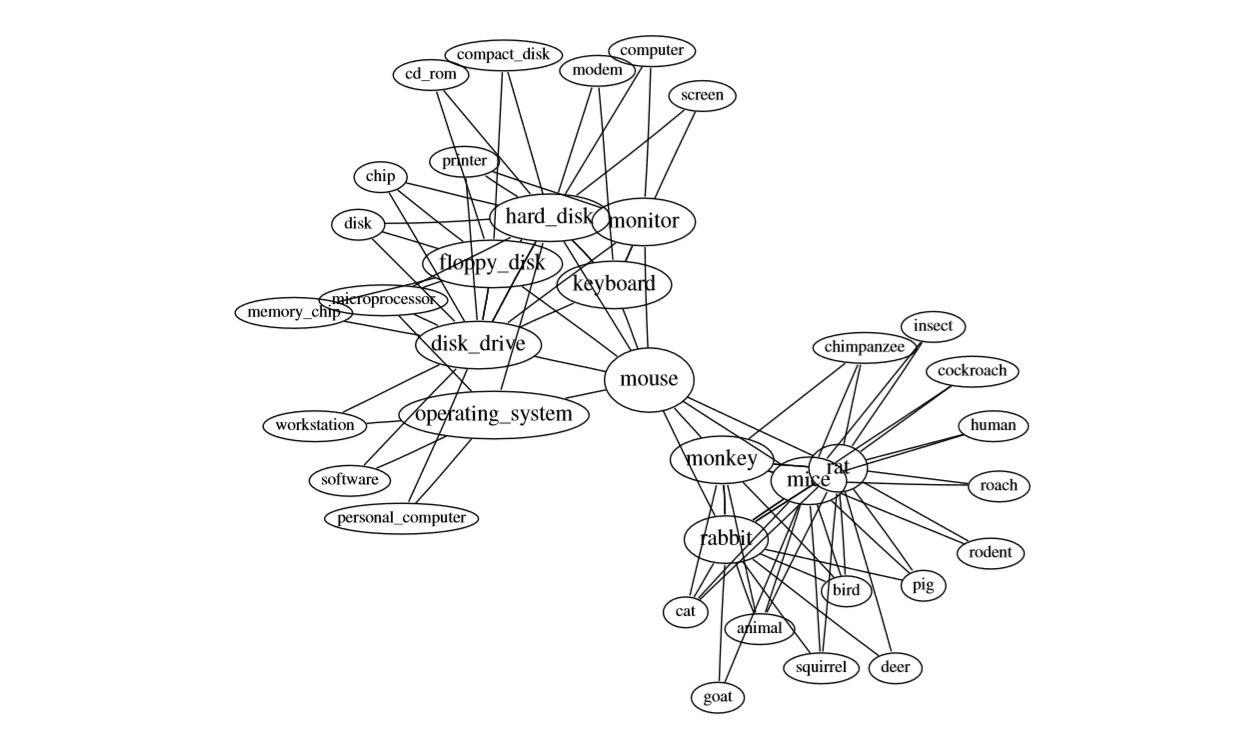
\includegraphics[width=0.8\linewidth]{widdows2.jpg}
	\captionof{figure}{\color{Green} Neighbours of the ambiguous word \textit{mouse} - Widdows 2004}
\end{center}\vspace{1cm}

\begin{itemize}
	\item 
	We will work around this issue using word sense disambiguation and studying consolidated approaches of this field to deal with this.\\
	
	\item To approach synonym extraction, we will use linguistic databases such as dictionaries and thesauri, as well as structured resources such as WordNet.\\
	
	\item Those DBs will be used to support models that differentiate between Synonym and other relationships of words.\\
	
	\item Classifiers like Naive-Bayes or Decision Tree will be used to explore neighboring word vectors and to identify synonymic relationships.\\
	%
\end{itemize}

%----------------------------------------------------------------------------------------
%	FORTHCOMING RESEARCH
%----------------------------------------------------------------------------------------

\section*{Forthcoming Research}

\begin{itemize}
	
	\item Define the models which are going to be used on the task.\\ 
	
	\item Develop a corpus to train and test synonym extraction models in Portuguese.\\
	
	\item Compare the results to point out limitations and areas to improve.\\
	
	\item Based on the knowledge about the nature of synonym and test results, develop a deep analysis on the possibility of automation of synonym extraction.\\
\end{itemize}

 %----------------------------------------------------------------------------------------
%	REFERENCES
%----------------------------------------------------------------------------------------

\nocite{*} % Print all references regardless of whether they were cited in the poster or not
\bibliographystyle{plain} % Plain referencing style
\bibliography{sample} % Use the example bibliography file sample.bib


%----------------------------------------------------------------------------------------

\end{multicols}
\end{document}